\chapter{Overview}\label{ch:overview}
The purpose of this chapter is to give an overview of the collected system so that the reader has a better idea of the purpose of each chapter in this thesis. Moreso, it is also to define exactly what the system is capable of doing and how it perceives and manipulates its environment. In the coming sections, the terminology of "the system" is explained, along with its capabilities for solving tasks. This information is carried into the subsequent sections, where the whole system is reviewed.

\section{Introduction to the system}\label{sec:sys_overview_task}
The full pipeline is named 'system' in this thesis. Figure \ref{fig:Full_pipeline_data_IN_OUT} presents a diagram describing the input and output of the system. The system is capable of receiving text as input, which is expected to be natural language. The input will have three distinct terms, as shown in figure \ref{fig:sentence_instruction_action}. The input sentence is the input the user passes to the system. The second term is 'instruction'. The instructions are all natural sentences in the input sentence. Instructions are used instead of the input sentence later in the thesis, as they have the feature that the root of the instruction is the verb used to determine the instructions actions. The terminology of word roots is explained in chapter \ref{ch:NLP}. The last terminology of the input is 'actions'. The actions are objects that are executable on the robot manipulator. Usually, the instructions contain only one action each. But because the action of grabbing does not require specification from the user, it is possible to combine it with the action to move, as shown in figure \ref{fig:sentence_instruction_action}.
\begin{figure}[ht]
    \centering
    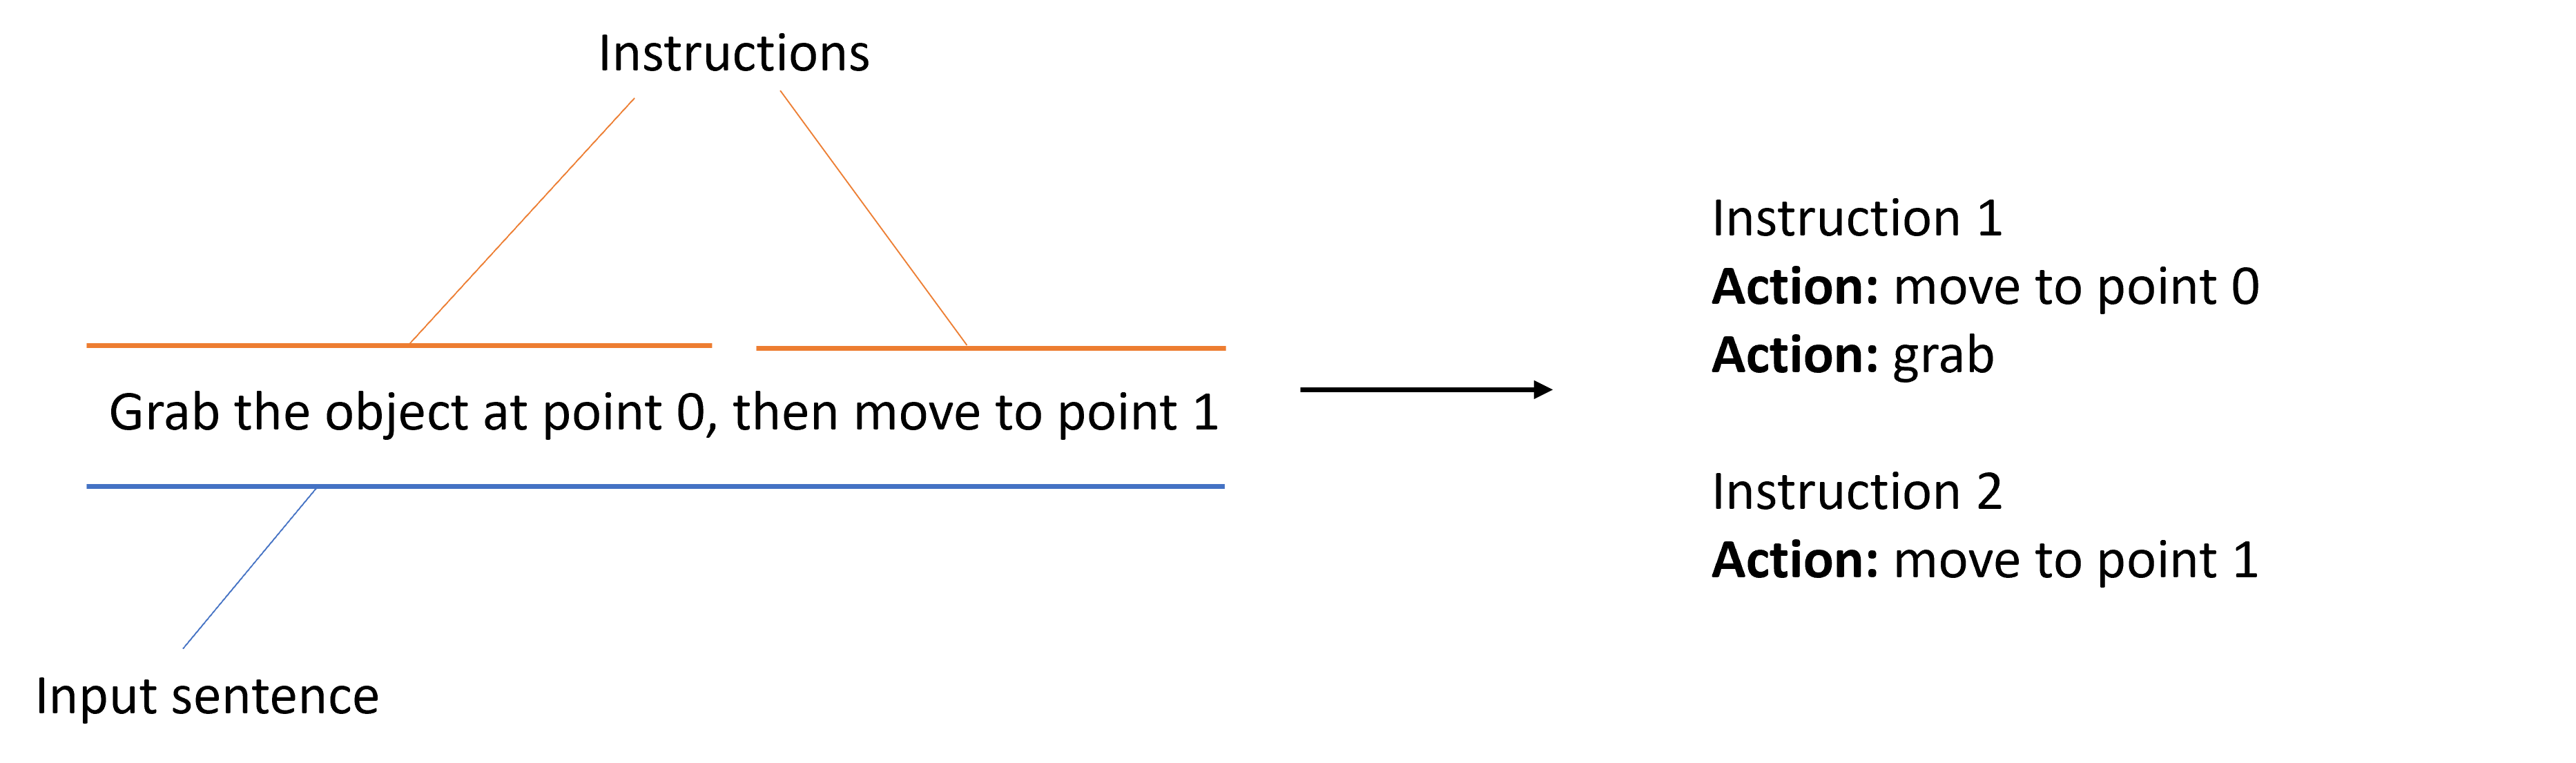
\includegraphics[width=13cm]{img/Sentence_instruction_action.png}
    \caption{Figure shows the relation between the terms input sentence, instructions, and actions.}
    \label{fig:sentence_instruction_action}
\end{figure}

The system works by using three sub-pipelines.
The interpretation of natural language is done by using natural language processing (NLP) tools. By using the NLP tools, the input can be split into its instructions. Moreso, NLP information regarding sentence structure and grammatical categories are also given. This part is named the NLP pipeline and is the first sub-pipeline of the system. Afterward, the parser analyzes the NLP output to figure out what actions the sentence consists of. This second sub-pipeline is called the parser pipeline. The output of the parser pipeline is a list of actions in sequence given to the third and final sub-pipeline. The third sub-pipeline is the kinematics pipeline, which handles the system's interaction with the environment. Mainly, it is used to move the UR5e robot according to the actions in the list. But it is not limited to only moving the robot. The kinematics pipeline is also responsible for placing points and frames in space and manipulating the robot gripper. Frames and points are information regarding pose and location stored in the database of the system. The next section delves deeper into the idea of points and frames.
\begin{figure}[ht]
    \centering
    
\includegraphics[width=13cm]{img/Full_pipeline_data_IN_OUT.png}
    \caption{Illustration of the information process given the full pipeline.}
    \label{fig:Full_pipeline_data_IN_OUT}
\end{figure}


\section{Frames and points}\label{sec:sys_overview_frames_points}
The positions stored in the database serve the purpose of supporting the UR5e robot so that it becomes easier for it to solve tasks. It is important to explain in detail what positions and frames are, and how the system operates using them. 

\begin{figure}
    \centering
    \begin{subfigure}[b]{0.3\textwidth}
        \centering
        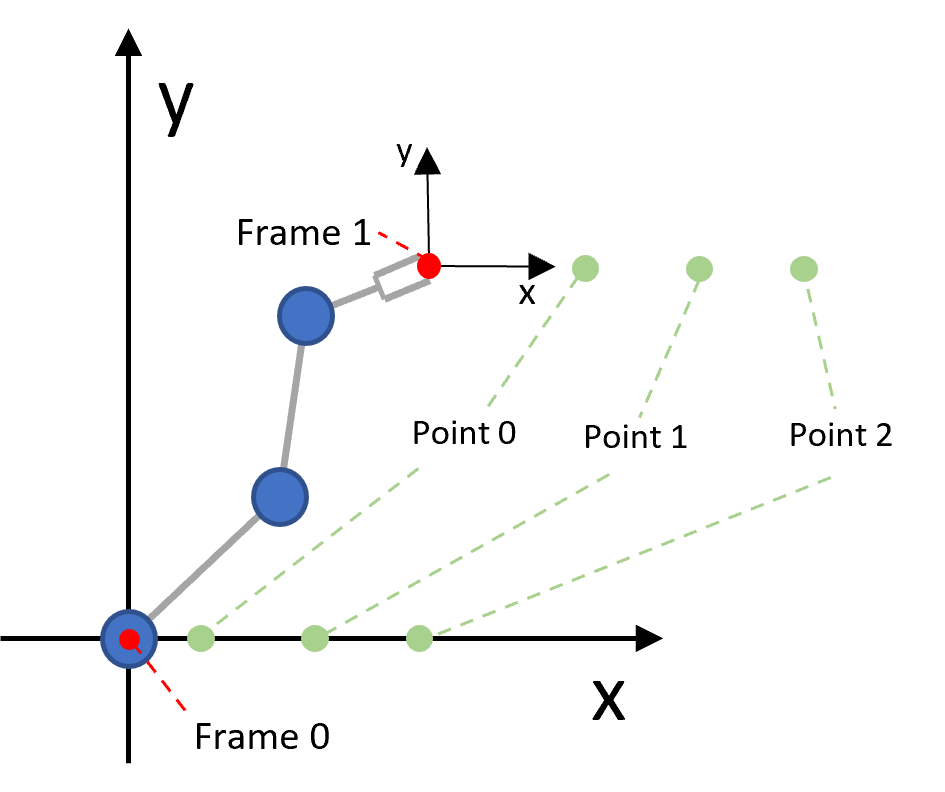
\includegraphics[width=6.5cm]{img/point_frame_explanation1.png}
        \caption{$ $ Visualization of points in frame 1.}
        \label{fig:overview__PF1}
    \end{subfigure}
    \hspace{3cm}
    \begin{subfigure}[b]{0.3\textwidth}
        \centering
        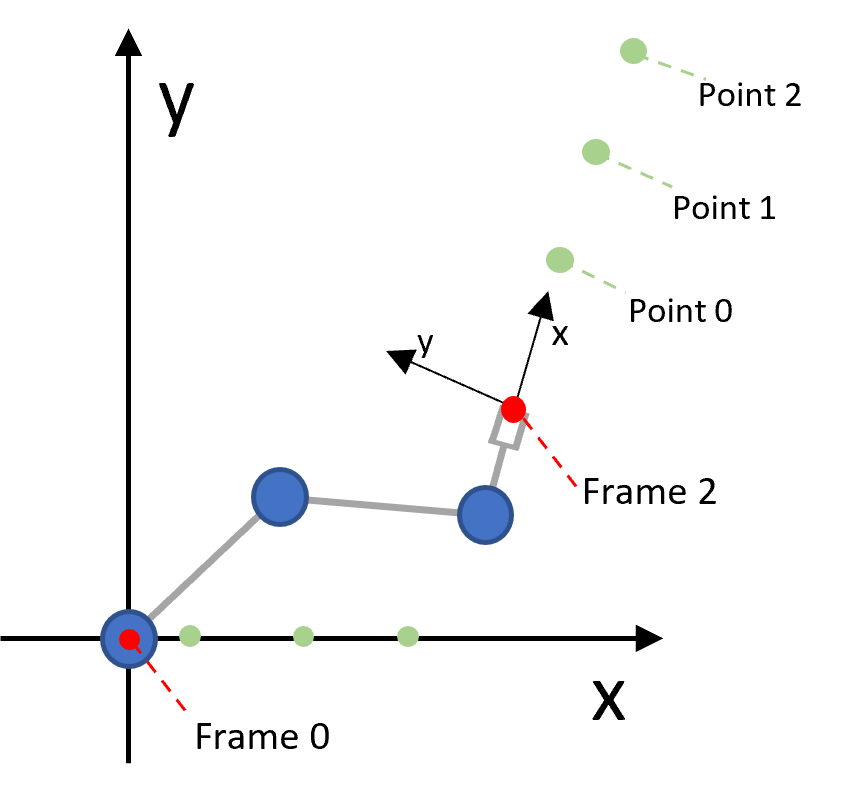
\includegraphics[width=6.5cm]{img/point_frame_explanation2.png}
        \caption{$ $ Visualization of points in frame 2.}
        \label{fig:overview__PF2}
    \end{subfigure}
       \caption{2D visualization of the point frame system created.}
       \label{fig:point_frame_explanation}
\end{figure}

Frames are coordinate systems set in space in reference to the base coordinate system. The base coordinate system is placed at the base of the robot. The purpose of the ability to set poses and frames online is to bring a coordinate system closer to the task operation field. This ability facilitates the robot's setup of the correct points in space. Figure \ref{fig:point_frame_explanation} shows a 2D visualization of how the points and frames are intertwined. 
Points set in the system are relative to coordinate systems. The figure shows how points 0, 1, and 2 are set in extension of the x-axis and are therefore apparent along the given axis in all of frames 0, 1, and 2. Subfigure 3.3.b shows that the feature allows the user to set points in a complex position, compared to trying to set them up in reference to the base frame (frame 0). Using frame 2, setting up the three points would be a task solved in 1 dimension only (the x-axis).
The system only sees one frame at a time. Meaning that all points in space are relative to the frame that the system is currently working on. So to change the working frame, the user must specify this action for the system. A language command example could be \textit{"Set frame 1 as the current frame"}. And to create new frames, the language command could be \textit{"Set position as a frame"}. This design makes the language control simpler, as the language processor does not need to process commands such as \textit{"Move to point 1 in frame 1"}.

\section{System interfacer}\label{sec:sys_overview_design}
The system interfacer is the interactional part, serving the purpose of communicating with the user. Given that the thesis revolves around natural language communication control, it naturally follows that the system interface is a terminal with no input constraint. This is shown in figure \ref{fig:overview__terminal}.

\begin{figure}[ht]
    \centering
    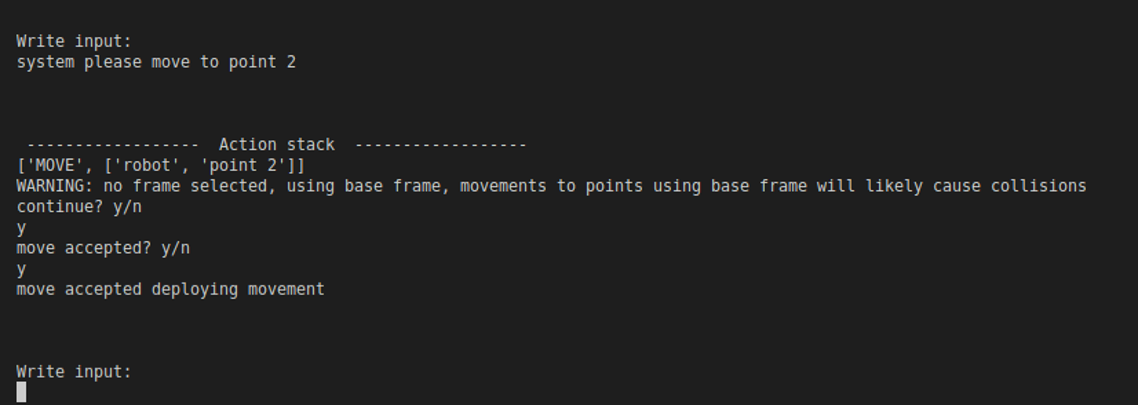
\includegraphics[width=13cm]{img/terminal_input.png}
    \caption{Input from the system after instructing it to move to point 2.}
    \label{fig:overview__terminal}
\end{figure}

In the given figure, it is shown that the interaction happens twice. The first time is a safety prompt, as it is unusual to move to any point while the robot is working in the base frame. It usually causes the robot to collide with itself as the base frame is placed at the base of the robot. This warning is ignored in this instruction to further show the second interaction. The second prompt is for user confirmation that the action stack is as desired. Further in the thesis, it is also shown that a simulation of the robot's movement is made to make sure that the movement is not erroneous.

\section{Natural language input constraints}
The natural language instructions used to control the system are only a subset of full natural language, as there are constraints made to simplify the task for this thesis. These constraints are mentioned in chapter \ref{ch:intro} as the constraints of the problem. This section delves deeper into how the system should act if the input is incomprehensible in any way. As an example, sentences such as \textit{"Do a funny dance"} cannot be successfully executed as they require contextual knowledge and advanced movements. The subset of instructions that the system is capable of are instructions that focus on simple sequential tasks, such as \textit{"Move to point 1, then move to point 2, then grip the object."}.
Therefore, though the interface can input arbitrary text, only a specific language style is converted into actions. If the user inputs instructions in any way that is incomprehensible to the system, it would either not output any actions, give a better explanation of why the instruction was not understood, or give a guess as to what the user might have meant. These options are explored in chapter \ref{ch:parser_pipeline}.

\section{Summary}
The system is a programmed pipeline, with a UR5e robot arm equipped with a gripper, capable of processing natural language such that it becomes capable of manipulating its environment using the robot. What has been covered as part of the overview is a short explanation of the purpose of the pipeline and each of its sub-pipelines, how the physical space is mapped with points and frames, and how the system is interacted with. The overview gives the reader information that will be used later to further explain how each sub-pipeline has been created. The next chapters of the thesis cover the theory and the creation of the sub-pipelines. 